%%%%%%%%%%%%%%%%%%%%%%%%%%%%%%%%%%%%%%%%%
% Journal Article
% LaTeX Template
% Version 1.4 (15/5/16)
%
% This template has been downloaded from:
% http://www.LaTeXTemplates.com
%
% Original author:
% Frits Wenneker (http://www.howtotex.com) with extensive modifications by
% Vel (vel@LaTeXTemplates.com)
%
% License:
% CC BY-NC-SA 3.0 (http://creativecommons.org/licenses/by-nc-sa/3.0/)
%
%%%%%%%%%%%%%%%%%%%%%%%%%%%%%%%%%%%%%%%%%

%----------------------------------------------------------------------------------------
%	PACKAGES AND OTHER DOCUMENT CONFIGURATIONS
%----------------------------------------------------------------------------------------

\documentclass[twoside,twocolumn]{article}

\usepackage{blindtext} % Package to generate dummy text throughout this template 

\usepackage[sc]{mathpazo} % Use the Palatino font
\usepackage[T1]{fontenc} % Use 8-bit encoding that has 256 glyphs
\linespread{1.05} % Line spacing - Palatino needs more space between lines
\usepackage{microtype} % Slightly tweak font spacing for aesthetics

\usepackage[german]{babel} % Language hyphenation and typographical rules

\usepackage[hmarginratio=1:1,top=32mm,columnsep=20pt]{geometry} % Document margins
\usepackage[hang, small,labelfont=bf,up,textfont=it,up]{caption} % Custom captions under/above floats in tables or figures
\usepackage{booktabs} % Horizontal rules in tables

\usepackage{lettrine} % The lettrine is the first enlarged letter at the beginning of the text

\usepackage{enumitem} % Customized lists
\setlist[itemize]{noitemsep} % Make itemize lists more compact

\usepackage{abstract} % Allows abstract customization
\renewcommand{\abstractnamefont}{\normalfont\bfseries} % Set the "Abstract" text to bold
\renewcommand{\abstracttextfont}{\normalfont\small\itshape} % Set the abstract itself to small italic text

\usepackage{titlesec} % Allows customization of titles
\renewcommand\thesection{\Roman{section}} % Roman numerals for the sections
\renewcommand\thesubsection{\roman{subsection}} % roman numerals for subsections
\titleformat{\section}[block]{\large\scshape\centering}{\thesection.}{1em}{} % Change the look of the section titles
\titleformat{\subsection}[block]{\large}{\thesubsection.}{1em}{} % Change the look of the section titles

\usepackage{fancyhdr} % Headers and footers
\pagestyle{fancy} % All pages have headers and footers
\fancyhead{} % Blank out the default header
\fancyfoot{} % Blank out the default footer
\fancyhead[L]{Raphael Drechsler} % Custom header text
\fancyhead[C]{Oberseminar Datenbanksysteme} % Custom header text
\fancyhead[R]{Sommersemester 2018} % Custom header text
\fancyfoot[RO,LE]{\thepage} % Custom footer text

\usepackage{titling} % Customizing the title section




\usepackage[utf8]{inputenc}
\usepackage{graphicx}

\usepackage{url}
\usepackage{breakurl}
\usepackage[breaklinks]{hyperref}
\def\UrlBreaks{\do\/\do-}

%----------------------------------------------------------------------------------------
%	TITLE SECTION
%----------------------------------------------------------------------------------------

\setlength{\droptitle}{-4\baselineskip} % Move the title up

\pretitle{\begin{center}\Huge\bfseries} % Article title formatting
\posttitle{\end{center}} % Article title closing formatting
\title{Data Lakes} % Article title
\author{%
\textsc{Raphael Drechsler}\\[1ex] % Your name
\normalsize HTWK Leipzig \\ 
\normalsize Fakultät Informatik, Mathematik und Naturwissenschaften\\ 
\normalsize Studiengang Informatik Master - Matrikelnr. 69872\\% Your email address
%\and % Uncomment if 2 authors are required, duplicate these 4 lines if more
%\textsc{Jane Smith}\thanks{Corresponding author} \\[1ex] % Second author's name
%\normalsize University of Utah \\ % Second author's institution
%\normalsize \href{mailto:jane@smith.com}{jane@smith.com} % Second author's email address
}
 \date{60.30.2018} % Leave empty to omit a date
\renewcommand{\maketitlehookd}{%
\begin{abstract}
\noindent 
Der Begriff des Data Lakes ist 2010 entstanden und wurde in den letzten Jahren stark ''gehyped''.\cite{src1} \cite{src2} \cite{src3} Es haben sich viele verschiedene Konzepte und Ansichten zum Thema entwickelt. Im Internet findet man bei einer Recherche zum Thema Data Lake von einem existierneden Unternehmen, welches sich ''the Data-Lake-Company'' nennt\cite{dlc}, bis hin zu einem Blogeintrag, der die Frage ''Are Data Lakes Fake-News?'' mit ja beantwortet\cite{src4} eine ganze Menge. Dabei wird die Frage danach, was ein Data Lake ist, von den verscheidenen Quellen nicht eindutig beantwortet. Auch gibt es zum Zeitpunkt des Erstellens dieses Dokumentes in der deutschsprachigen Wikipedia nock keinen Eintrag zu diesem Thema. Die Motivation dieses Abstracts besteht also darin, die bestehenden Unklarheiten zu beleuchten; zu klären was ein Data-Lake ist und sich mit der Frage ''Are Data Lakes Fake-News'' auseinanderzusetzen.
\end{abstract}
}

%----------------------------------------------------------------------------------------

\begin{document}

% Print the title
\maketitle

%----------------------------------------------------------------------------------------
%	ARTICLE CONTENTS
%----------------------------------------------------------------------------------------

\section{Definitionsfrage ''Data Lake''}
\lettrine[nindent=0em,lines=2]{D}er Begriff des Data Lakes wurde erstmalig von James Dixon (CTO von Pentaho \footnote{Pentaho gehört seit September 2017 dem Unternehmen Hitachi Vantara an}) geprägt. Auf seinem Blog \cite{src5}  und in mehren auf Youtube veröffentlichten Videos \cite{src6} stellt Dixon damals die von Pentaho angebotene Hadoop-basierte Big-Data-Lösung vor. Im Rahmen dieser Vorstellung stellt er auch das Prinzip vor, auf welchem die Solution basiert: Den Data Lake.\\
Dixon's Erläuterung des Prinzips beginnen damit, dass er durch Pentaho betrachtete Big-Data-Szenarien betrachtet und folgende gemeinsame Eigenschaften ableitet. 
\begin{itemize}
	\item Es liegt ein großes Datenvolumen vor, welches zu analysieren ist
	\item Die Daten entspringen einer Quelle
	\item Die Daten liegen in ihrer rohen Form vor \textit{(können also strukturiert, semi-strukturiert und un-strukturiert sein)}
	\item ggf. sind die Daten angereichert \textit{(bspw. Anreichern von Weblogs um Geocodes)}
\end{itemize}

\noindent Liegt ein Daten-Volumen vor, auf welches diese Eigenschaften zutreffen, handelt es sich Dixon nach um einen Data Lake. Im Weiteren nennt Dixon zusätzliche Eigenschaften eines solchen Data Lakes. Im Kern der Betrachtung steht dabei, dass der Data Lake als Datenvolumen verschiedenen Anwendern über verschiedene Unternehmensbereiche bekannte und unbekannte (wenn auch kleinere) Fragen beantworten kann und es daher sinnvoll ist, dieses Datenvolumen für spätere Analysen abzuspeichern.\\
Der von Dixon ausgeführte bildliche Vergleich macht diesen Umstand und die Vorstellung davon, was ein Data Lake ist, noch deutlicher.

\begin{figure}[h]
	\centering 
	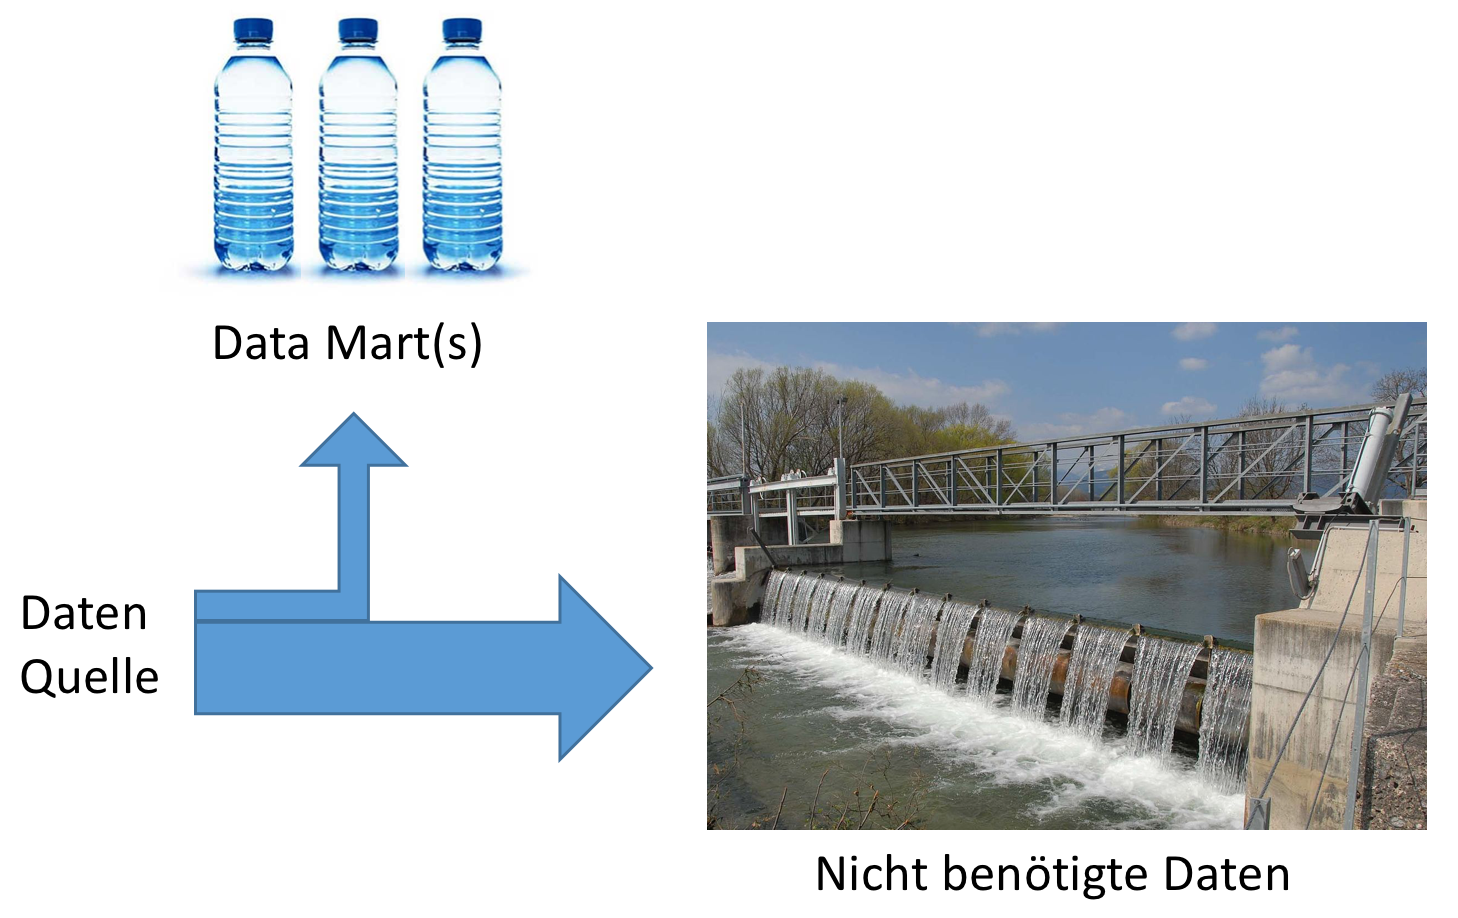
\includegraphics[width=0.4\textwidth]{img/p1} 
	\caption{Data Marts als Wasserflaschen \textit{nach} \cite{src6}}	
\end{figure}

Die Verbildlichung setzt bei den Data Marts an und stellt diese als fertig abgefüllte Mineralwasser-Flaschen dar. Das Wasser für diese Flaschen wurde aus einer Datenquelle gewonnen, bereinigt, aufbereitet und für den finalen Verwendungszweck abgepackt. Der Teil des Wassers (der Großteil), welcher nicht in die Data Marts eingegangen ist, fließt einfach ab. (Siehe Abb. 1)\\
Das Konzept des Data Lakes setzt an dieser Stelle an. Unter der Annahme, dass auch der Teil der Daten, welcher abfließt, wertvolle Informationen enthalten kann, wird das Datenvolumen als Data Lake persistiert. Aus diesem lassen sich die Data Marts beliefern. Zusätzlich ist es durch das Speichern möglich, per Ad-Hoc-Query oder Report direkt auf das Datenvolumen zuzugreifen und somit zuvor unbekannte Fragen beantworten zu können. Zudem können Data Lakes wiederum als Datenquellen für Data Warehouses genutzt werden. Es ergibt sich das folgende Bild:
\begin{figure}[h]
	\centering 
	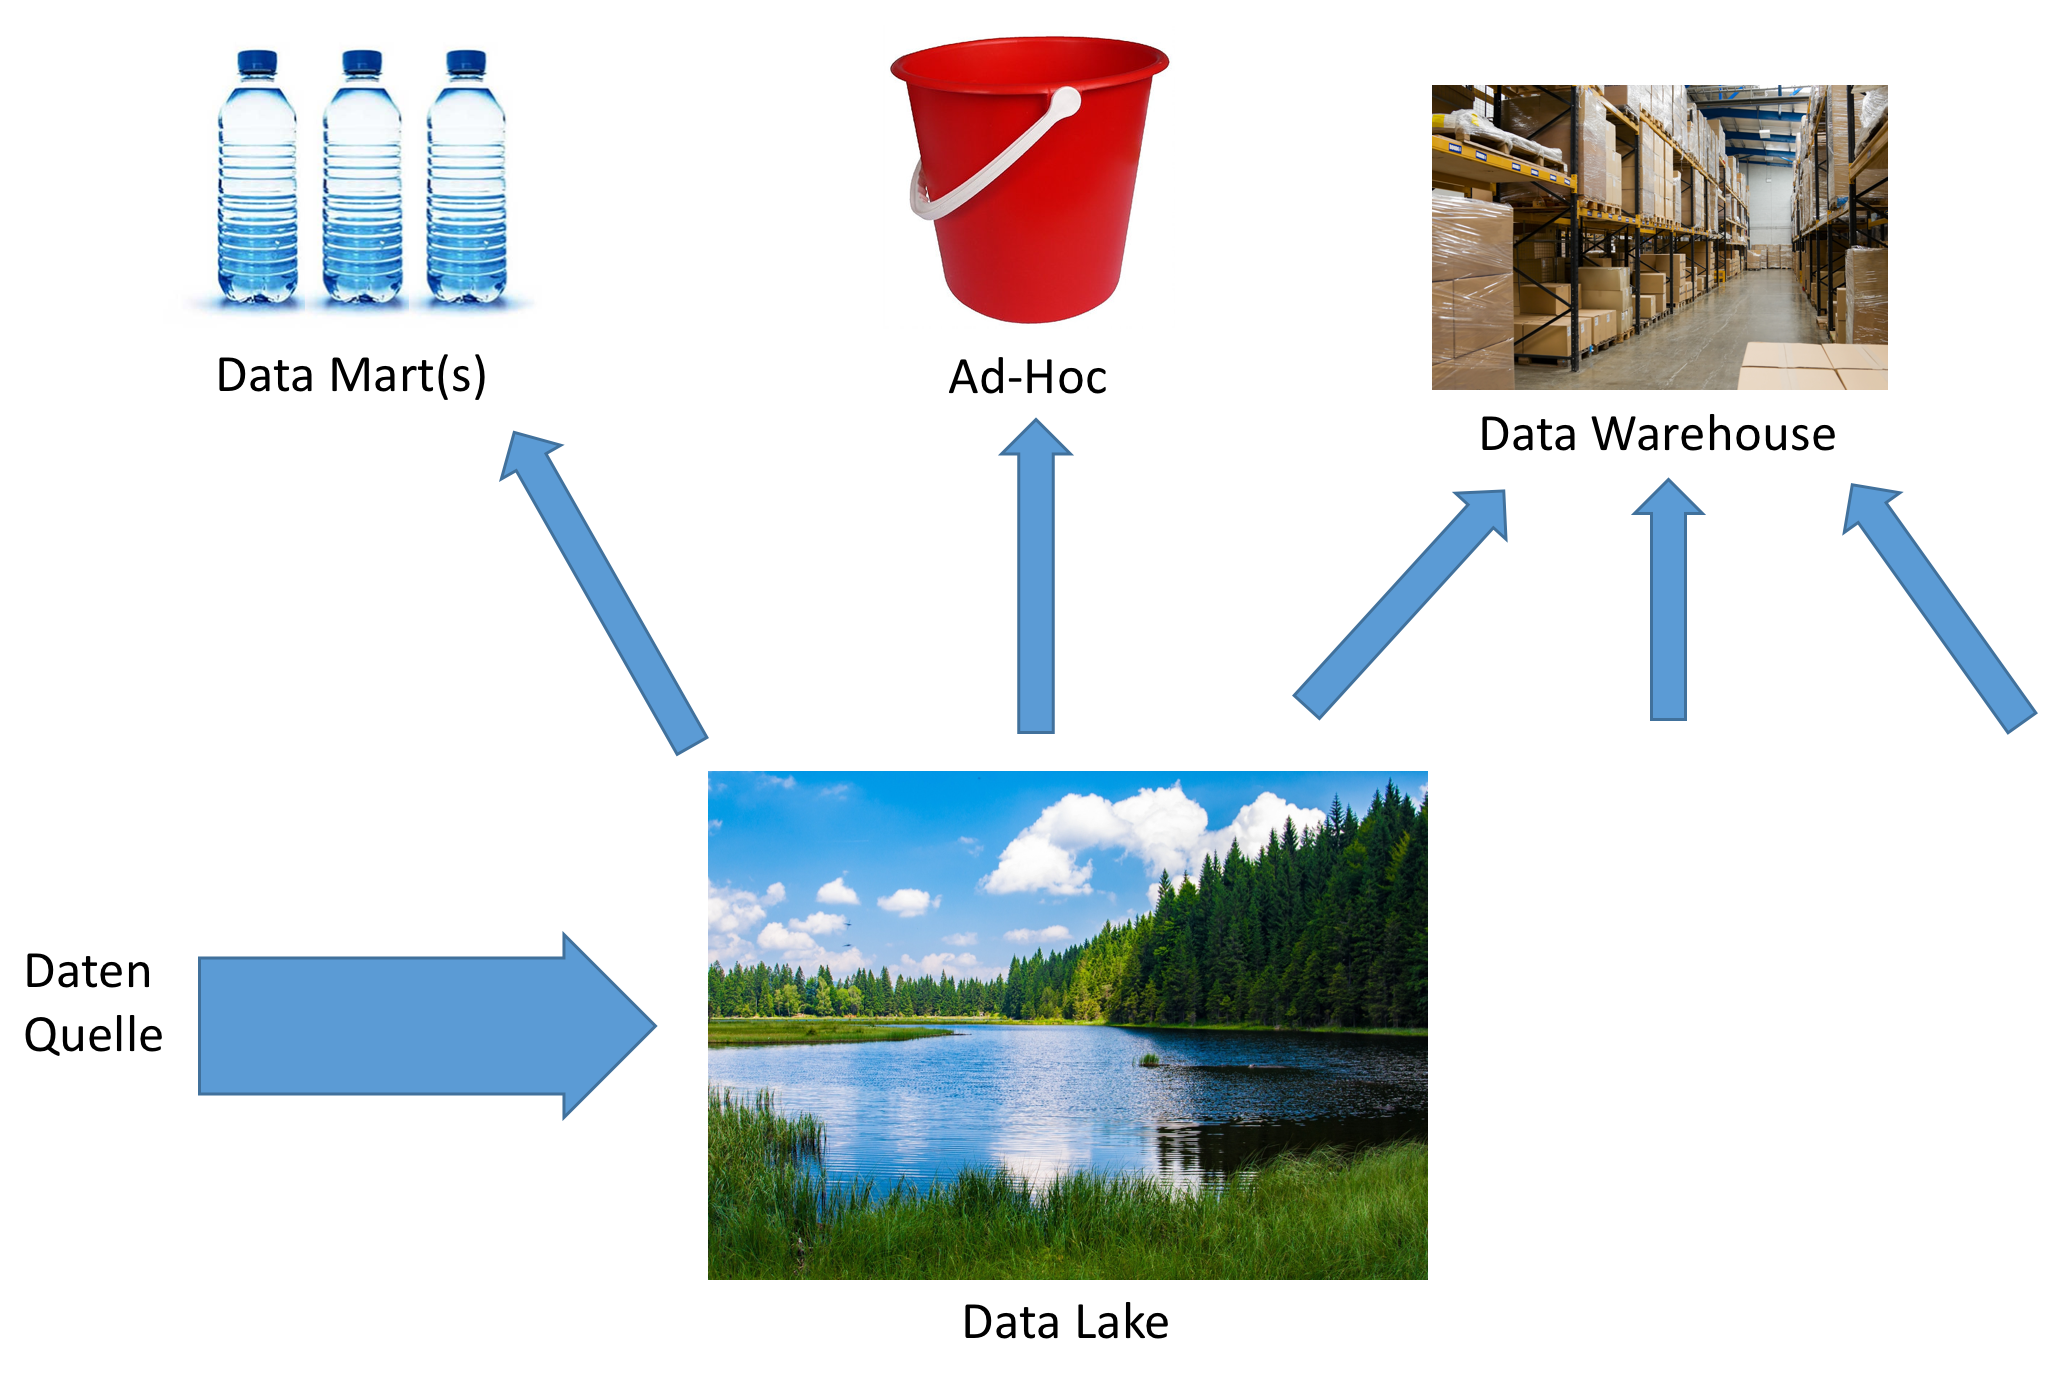
\includegraphics[width=0.4\textwidth]{img/p2} 
	\caption{Verbildlichung des Data Lakes \textit{nach} \cite{src6}}	
\end{figure}

\noindent Diesem Prinzip folgend stellt Dixon die folgende Architektur der Pentaho-Solution vor.
\begin{figure}[h]
	\centering 
	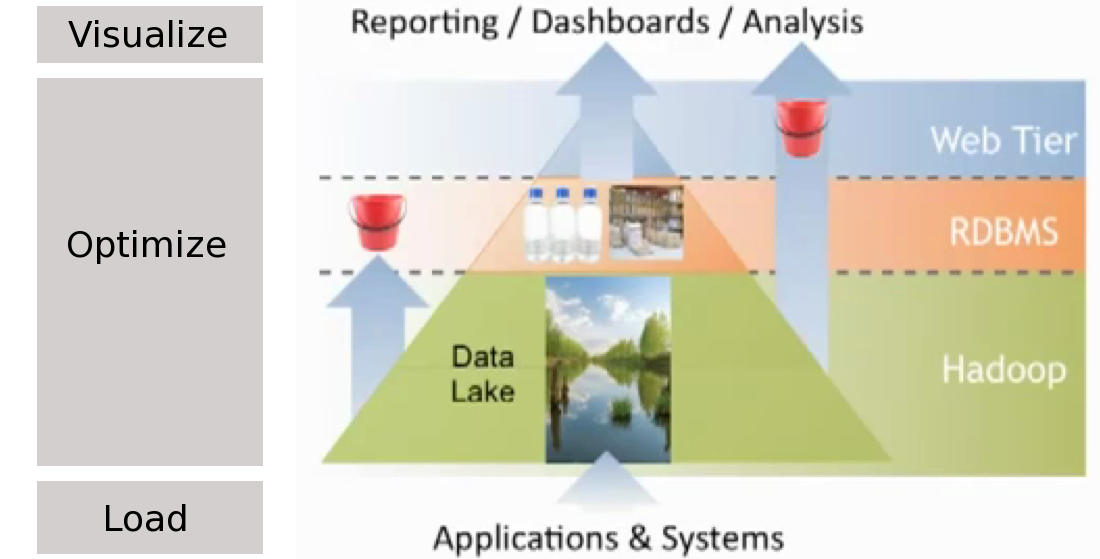
\includegraphics[width=0.47\textwidth]{img/p3} 
	\caption{Architektur Pentaho-Solution 2010 \cite{src6b}}	
\end{figure}

\noindent Dabei finden sich die Elemente des Prinzips in den drei Schichten der Architektur (Load, Optimize und Visualize) wieder.\cite{src6}\cite{src6b} \\
Im weiteren Verlauf der Video-Strecke zur Solution geht Dixon auf die einzelnen Komponenten und deren Funktionsweisen ein. Im Wesentlichen ist die Definition des Data Lakes durch Dixon bzw. Pentaho an diesem Punkt abgeschlossen.\\
Da die Definition einigen Raum für Interpretation lässt, wurde der Begriff im Laufe der folgenden Jahre von verschiedenen Seiten unterschiedlich aufgefasst und teilweise neu interpretiert. Heute gibt es keinen einheitlichen Begriff des Data Lakes mehr.\cite{src7}

\section{Wie funktioniert ein Data Lake?}
Über die verschiedenen Lösungen und Konzepte, die zu Data-Lake-Solutions existieren, gibt es einige Gemeinsamkeiten. Diese sollen im folgenden betrachtet werden.

\paragraph{Aufbau und Workflow}
Der Aufbau einer Data-Lake-Solution ist zu der von Dixon dargestellten Architektur analog.
Die Architektur besteht aus den folgenden drei Schichten.\cite{src8} \cite{src9}
\begin{itemize}
	\item Data Sources: \textit{Umfasst die Quell-Systeme bzw. Data-Streams inkl. der Daten, die das Daten-Volumen (den Data Lake) bilden}
	\item Processing and Storage-Layer: \textit{Schicht zum Speichern und weiterverarbeiten des Daten-Volumens/Data Lakes} 
	\item Visualisation-Layer: \textit{Schicht in welcher die Daten aus dem DWH visualisiert werden oder/und eine Oberfläche für das Abfragen von Ad-Queries bereitgestellt wird. Weitere Komponenten und Formen der Visualisierung sind hierbei denkbar.}
\end{itemize}

Dabei wird die Processing and Storage-Layer gelegentlich als der Data Lake bezeichnet (vgl. bspw. \cite{mdb}), was von Dixons Definition des Data Lakes als Datenvolumen (und nicht als Speicherort) abweicht.\\


Der Workflow in einer Data-Lake-Solution lässt sich wie folgt skizzieren. Dabei können die der Processing and Storage-Layer nachgelagerten Komponenten je nach betrachteter Solution variieren.

\begin{figure}[h]
	\centering 
	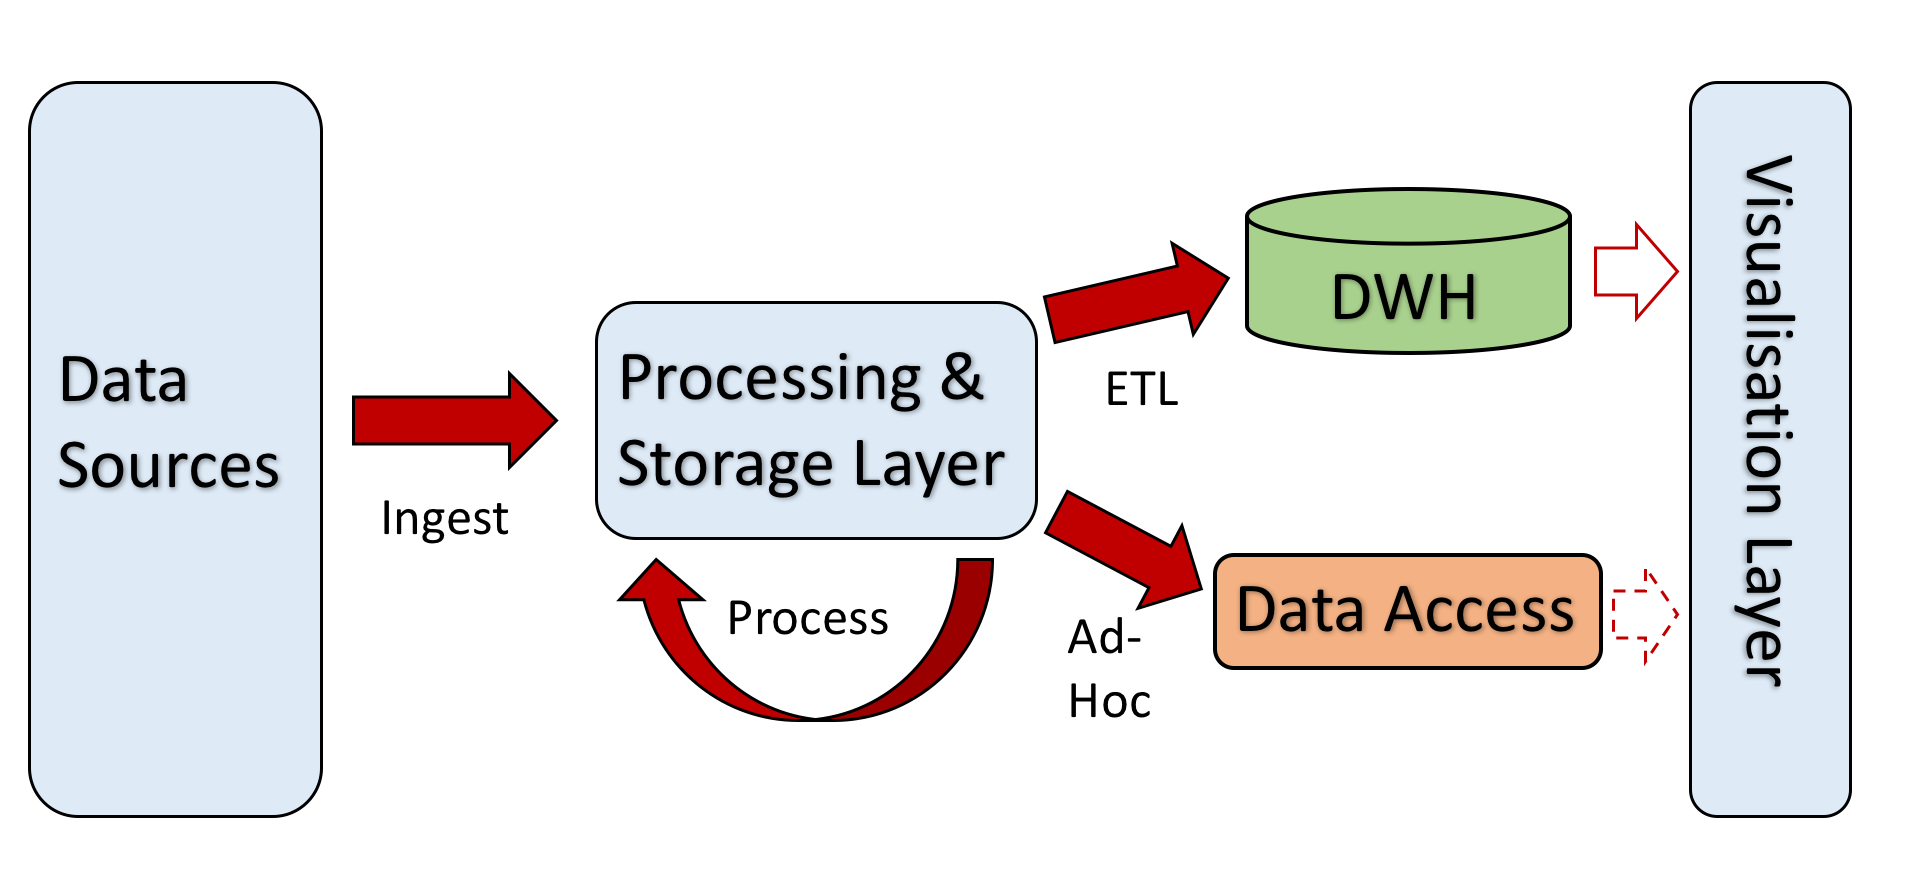
\includegraphics[width=0.4\textwidth]{img/p4} 
	\caption{DRT \textit{nach} \cite{src9}}	
\end{figure}

Die Daten durchlaufen in diesem Prozess die folgenden Schritte.
\begin{itemize}
	\item Ingestion: \textit{(engl. für Aufnehmen). Die Daten werden aus den Quell-Systemen bzw. Data-Streams in die Processing and Storage-Layer geladen.}
	\item Processing: \textit{Das persistierte Datenvolumen wird so weit aufbereitet, dass es für Analysen, Abfragen und schließlich Reports verwendet werden kann. Diese Aufbereitung obliegt der Rolle des sogenannten Data Scientist.\cite{src8}} 
	\item Bereitstellung für konsumierende Systeme \textit{Die aufbereiteten Daten werden nun den nachgelagerten Systemen bereitgestellt.}
\end{itemize}
Wie sich an diesen Prozess die Visualisierung anschließt variiert - je nach eingesetzten Komponenten - von Solution zu Solution.\\

Im Folgenden sollen einige Detailfragen, die die Beschaffenheit der Komponenten einer Data-Lake-Solution und deren Zusammenspiel betreffen, näher beleuchtet werden.

\paragraph{Storage}
		Für das Speichern des Data Lakes (Datenvolumens) bestehen die Anforderungen, dass zum Einen alle Daten gespeichert werden und dass zum Anderen die Daten getreu Dixon's Definition in Rohform abgelegt werden müssen. Da daher sowohl strukturierte, semi-strukturierte und un-strukturierte Daten gespeichert werden müssen, ist eine sinnvolle Speicherung der Daten in einem RDBMS, welches vor dem Schreiben von Daten in die DB ein Schema voraussetzt (''Sceama on Write''), nicht möglich. Eine Lösung hierbei bietet der ''Sceama on Read''-Ansatz, bei dem jegliche Daten ohne definiertes Schema gespeichert werden und das Schema erst beim Lesen aus der DB über die Querys definiert wird.\\
		Apache Hadoop folgt diesem Ansatz und hat sich als On-Premise-Speicher für Data-Lake-Solutions durchgesetzt. Es existieren auch Online-Speicher für Data-Lakes, welche auf Hadoop basieren (Google Cloud Platform, Amazon S3, Azure Data Lake).
		\cite{src8}
\paragraph{Ingestion}
		Für das Aufnehmen der Daten in die Processing and Storage-Layer ist es erforderlich, dass Daten auf jede Art (via Batch oder Streaming) aufgenommen werden können. Apache bietet für beide Arten der Datenaufnahme entsprechende Processing-Systeme an. Als Beispiele seien hier Apache MapReduce, Squoop und Spark als Batch-Processing-Systeme und Apache Flink, Storm und Flume als Streaming-Systeme genannt.\cite{src8}\\
		Für den Fall, dass im Rahmen der Informationsgewinnung aus dem Data Lake Echtzeiteinsichten bezüglich Streams gewünscht sind, gilt es einen Konflikt zu lösen, der zwischen Verfügbarkeit und Konsistenz der Daten besteht. Die Stream-Daten müssen für spätere Auswertungen im Data-Lake persistiert werden, was jedoch Zeit kostet und die Möglichkeit auf Echtzeiteinsichten verwehrt. Durch den Einsatz einer Lambda-Architektur lässt sich dieser Konflikt dadurch auflösen, dass ein Batch-Processing-Tool (die Batch-Layer) eine Serving-Layer mit Daten beliefert. Eingehende Anfragen werden zu großen Teilen aus dieser Serving-Layer bearbeitet. Das Delta zur Echtzeitinformation wird durch ein zweites, parallel laufendes Streaming-Tool (der Speed-Layer) aufgefüllt. Somit ist sowohl das Persistieren der Daten als auch eine Echtzeitauswertung möglich. \cite{src10} \\
		
		BILD ZU LAMBDA\\
		
		Eine Alternative zur Lambda-Architektur bietet die Kappa-Architektur. In dieser wird lediglich ein Stream-basiertes Processing-Tool eingesetzt. Dieses ist im Fall einer fehlerhaften Verarbeitung in der Lage mit teilweise persistierte Daten einen sogenannten ''Replay'' auszuführen. Dabei wird ein paralleler Streaming-Job gestartet, bis der Fehler ausgeglichen ist. Dies bietet den Vorteil, dass die entsprecheden Jobs für die Verarbeitung nur noch mit einem Tool implementiert werden müssen.\cite{src11} \\
		Die Tools für die Datenaufnahme sowie die Lambda- bzw. Kappa-Architektur finden auch in den späteren Prozessen des Workflows (insbesondere Process und ggf. Consumption) Anwendung.
		
\paragraph{Process}
		Sind die Daten in den Data-Lake gelangt, muss der Datensee für die Verwendung aufbereitet werden. Die entsprechenden Arbeiten werden von einer Rolle ausgeführt, die im Konzept des Data-Lakes als Data-Scientist bekannt ist.
		Der Data-Scientist muss zunächst die Daten untersuchen. Er führt ein Profiling der Daten durch und hält seine Ergebnisse sinnvollerweise in einem Metadaten-Katalog fest. Hierbei ist es wichtig zu verstehen, worum es sich bei den vorliegenden Daten handelt, wie ihr ursprüngliches Schema war und wie dich die Daten aus verschiedenen Quellen integrieren lassen. Diese Vorbereitung ist notwendig, um getreu dem ''Schema on Read''-Ansatz nun ein sinnvolles Schema für das Lesen der Daten definieren zu können.\\
		Anschließend kann die Analyse der eigentlichen Daten und daraufhin die Bereitstellung der Daten für das Konsumieren erfolgen. Dabei können über den gesamten Arbeitsschritt des Processings mehrere Iterationen notwendig sein, um einen Mehrwert in Form eines Informationsgewinnes zu erzeugen.\\
		Ist ein Mehrwert erzeugt worden, ist es im Hinblick auf die hinzukommenden Daten sinnvoll die auf die Daten angewandten Operationen als sogenannten WorkFlow zu arrangieren und diesen WorkFlow periodisch oder Ereignisgesteuert auf die Daten anzuwenden.\\
		Ebenfalls kann es dem Data-Scientist von Nutzen sein wiederkehrende, zusammenhängende Operationen als sogenannten DataFlow zu arrangieren, und diese DataFlow künftig als Tools für das Vorbereiten und die Analyse der Daten zu nutzen.\\
		\cite{src8}\cite{src12}
		%Weitere mögliche Aufgaben für den Data-Scientsit können die Optimierung der Performance und der 
		%Opt: Auch überlegen ob Codierung zu colum seperated Files oder Einsatz von NoSQL DB als intergraler Bestandteil von P und S. %Ggf. Mehr Administrationsaufwand und Speicher aber auszahlen in Zugriffsgeschwindigkeit und Zugriffsmöglichkeiten.
		
\paragraph{Consumption}
		In diesem Abschnitt des Workflows ist zu überlegen, welche Tools die aufbereiteten Daten aus dem Data Lake konsumieren wollen. Es können beispielsweise ..,..,.. beliefert werden.
		Zusätzlich ist in diesem Bereich zu überlegen, ob BI Tool auf DM oder DWH.
		Zudem Self-Service für Anfragen auf Data-Lake. Web-Oberfläche für alle Benutzer? Hier spielen Aspekt wie sehr technisch versiert so ein Benutzer.
		An sich Solution-Abhängig was für konsumierende Tools im Einsatz und wie konzept wer alles auf DL zugreift. Selfservice.\cite{src8}\cite{src12}
\paragraph{Monitoring}
		Einsatz von Moniitoring-Tool wie Apache Ambari zum Überwachen der Systemlandschaft.\cite{src8}
\paragraph{Data Governance}
		Umfasst ein großes Umfeld und ist in Data Lake ein wunder Punkt. Hierzu im folgenden Abschnitt mehr.


\section{Data Swamps: Kritik am Data Lake}
Welche Kritikpunkte am Data-Lake-Konzept bzw. an Data-Lake-Solutions bestehen, wird deutlich, wenn man die existierenden Verbildlichungen von pathologischen Data Lakes betrachtet.
\begin{itemize}
	\item Der Data Lake als Sumpf: \textit{Der gespeicherte Data Lake ist nicht zu durchschauen und die Aufbereitung zu abgepackten Mineralwasserflaschen ist unverhältnismäßig aufwendig bis unmöglich.\cite{src3}}
	\item Der Data Lake als Finnische Seenplatte:  \textit{Der Data Lake ist stark heterogen. Die aus mehreren Quellen im Data Lake vereinigten Datenmengen bilden mehrere voneinander abgetrennte Teil-Seen die nur schwer oder nicht zu integrieren sind\cite{src13}} 
	\item Der Data Lake als Flohmarkt: \textit{Hier findet man alles. Es stellt sich jedoch die Frage, wie man effizient sucht und welche Qualität die angebotenen Waren (Daten) haben.\cite{src12}} 
\end{itemize}

Gartner \footnote{Gartner Inc. - Marktforschung und Analyse von IT-Entwicklungen} beschreibt den Hype von Data Lakes darin begründet, dass das Konzept scheinbar eine Antwort auf die Frage nach mehr Agilität und Verfügbarkeit von Datenanalysen darstellt. Jedoch sei das Konzept lückenhaft. So kritisiert Gartner im Bericht \textit{''The Data Lake Fallacy: All Water and Little Substance.''}, dass das Aufnehmen sämtlicher Daten aus mehreren Quellen zu einem Data Lake führt, für den sich die benötigten Metadaten nicht ohne Weiteres erstellen oder gewinnen lassen, wodurch die gesammelten Daten ihren Wert verlieren. Zudem führt Gartner als wesentlichen Kritikpunkt an, dass das Konzept Data Lake keine Vorgaben zum Thema Data Governance macht.\cite{src3}

James Dixon bezieht 2014 zu dieser Kritik Stellung. Hierbei wird besonders ersichtlich, dass das von Gartner kritisierte Konzept einer Data-Lake-Solution von seiner ursprünglichen Definition aus dem Jahre 2010 abweicht. \cite{src14} So weist Dixon insbesondere darauf hin, dass der Data Lake nach seiner ursprünglichen Definition exakt eine Daten-Quellen akzeptiert und verweist für eine Solution, die mehrere Datenquellen aufnimmt, auf den sogenannten Wassergarten und die entsprechende Wassergartenarchitektur.\cite{src15} Bezüglich der fehlenden Metadaten merkt Dixon an, dass zum Data Lake nicht zwingend keine Metadaten vorliegen müssen. Genauer geht Dixon an dieser Stelle nicht auf die kritisierten Punkte ein, weswegen sich sie Kritik an einer ungenauen, lückenhaften Definition hält.

Sean Martin (Cambridge Semantics\footnote{Firma für Big-Data-Management und explorative Datenanalyse mit Sitz in Boston, Massachusetts}) beschreibt, dass viele Firmen sämtliche Daten, in der Hoffnung sie später nutzen zu können, in Hadoop speichern. Jedoch verleiren Sie anschließend den Überblick darüber, was alles gespeichert ist.
Bei einem Blick in die Praxis ist festzustellen, dass diese Gefahr einen Data-Swamp zu erzeugen bekannt geworden ist und sich daher ein Trend etabliert hat: Vorsichtiger werden. Primäre Aufgabe einer Data-Lake-Solution ist es nicht mehr alle Daten in Hadoop zu speichern. Stattdessen liegt der Fokus nun drauf, aus der gespeicherten Datenmenge einen Mehrwert zu erzeugen und nicht in der Datenmenge unterzugehen. \cite{src1} Diese Entwicklung kann als Paradigmenwechsel aufgefasst werden, da die neue Herangehensweise vom ursprünglichen Konzept (Alle Daten -wenn auch von nur einer Quelle- speichern) abweicht.

In jedem Fall rücken Data Governance und insbesondere die Beachtung der Metadaten als Schlüssel zu einer erfolgreichen Data-Lake-Solution in den Fokus. Dabei sind Data-Catalogue-Tools (Beispielsweise \textit{Smart Data Catalog von Waterline} und \textit{AWS Glue}) und spezielle Tools für Data Governance (wie \textit{Apache Atlas} und \textit{Cloudera Navigator}) sinnvolle Tools, um die für Data Governance relevanten Themen wie Data Lineage, Meatadaten-Suche, Datenqualität, Data Lifecycle-Management, Data Security und Data Integration anzugehen.\cite{src8}

\section{Fake-News! Existieren Data Lakes überhaupt?}
Uli Bethke (CEO von Sonra\footnote{Unternehmen für IT und Services mit Sitz in Dublin}) stellte August 2017 in einem Blogeintrag\cite{src4} die Frage ''Are Data Lakes Fake-News?'' und beantwortete Sie mit ja. Das soll als Motivation dienen, um abschließend die Frage zu untersuchen, ob Data Lakes überhaupt existieren.\\

Nach einer kurzen Recherche im Internet lassen sich einige Firmen finden, welche Solutions anbieten, die den Gegenstand ''Data Lake'' im Titel tragen. Unter anderem zu nennen sind: HVR, Podium Data, Snowflake, Zaloni\cite{c1}, Hitachi\cite{c2} und Hortonworks\cite{c3}.

Auch bei einer Suche nach erfolgreich umgesetzten Data-Lake-Solutions liefert Ergebnisse. 
Zu nennen sind hierbei beispielsweise die Success-Storys der Unternehmen Nissan\cite{s1}, UC Irvine Health\cite{s2} und Pinsight Media\cite{s3} als Kunden von Hortonworks. Auch auf der Website von Zaloni - ''the Data Lake Company'' finden sich kurze, positive Statements der Kunden CDS Global und Enterprise Strategy Group bezüglich der umgesetzten Lösungen.\cite{s4}.\\

Die wesentliche Frage ist jedoch, ob all diese umgesetzten und angebotenen Lösungen das Label einer Data-Lake-Solution tragen sollten. In wie Fern folgen die Lösungen dem ursprünglichen Konzept von Dixon bzw. Pentaho? In wie Fern weichen Sie davon ab? Und ist das ausschlaggebend dafür, dass eine Solution als Data-Lake-Solution gilt? Kurzum: Ohne genaue Definition der Begriffe Data-Lake und Data-Lake-Solution ist es nicht zweifelsfrei möglich Solutions diesen Begriffen unterzuordnen.\\
Zu einem ähnlichen Schluss kommt auch der Blogeintrag ''Are Data Lakes Fake-News?''. Hier heißt es, dass der Begriff ''Data Lake'' einige nützliche Konzepte (Data Reservoir und self-service analytics) fasst, jedoch letzenendes zu einer ''cath-all-phrase'' für alle Lösungen geworden ist, die nicht zum Thema Data-Warehousing gehören.\cite{src4}\\

Es ist also festzuhalten, dass Lösungen, die der grundlegenden Idee des Data Lakes folgen, existieren. Ob eine solche Solution aus diesem Grund das Label Data-Lake-Solution tragen sollte und welcher Mehrwert sich daraus ergibt obliegt der Einschätzung des Betrachters.


%------------------------------------------------


%------------------------------------------------



%----------------------------------------------------------------------------------------
%	REFERENCE LIST
%----------------------------------------------------------------------------------------

\bibliographystyle{unsrt}
\bibliography{bib.bib} % The file containing the bibliography

%----------------------------------------------------------------------------------------

\end{document}
